\documentclass[../classical_mechanics.tex]{subfiles}

\begin{document}

    \section{Polar Coordinates in 2D}
        \paragraph{}
        We have studied in great detail the mechanics of objects travelling in straight lines.
        Now we want to extend this to more general situations where objects can move along curved paths.
        We will first study motion in 2D as it is much simpler than 3D.
        As we saw in section~\ref{sec:motion-in-2-3d}, vectors in 2D can be equivalently described by two cartesian components or their length together with the angle they make with the $x$-axis.
        Depending on the type of motion in the problem, it is much simpler to describe the trajectory of an object the latter way.
        These are known as \textbf{polar coordinates}.

        \paragraph{}
        To set up the coordinate system, we define two new coordinate axes relative to the position vector $\vec{r}$.
        The first axis points along the direction of the position vector, and the second points one quarter turn anticlockwise from the first.
        These axes get two orthonormal vectors to form a basis which we label $\uvec{r}$ and $\uvec{\theta}$ respectively.
        \begin{figure}[H]
            \centering
            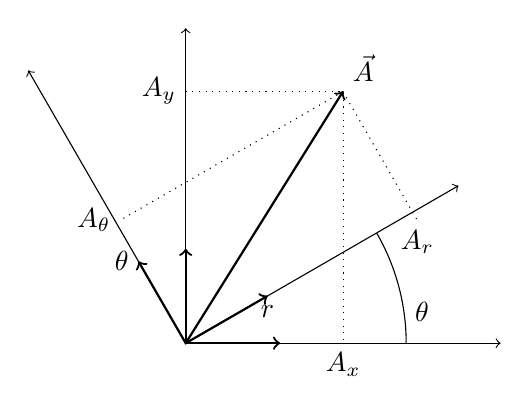
\begin{tikzpicture}[scale=4]
                \draw[<->] (0,1) |- (1,0);
                \draw[<->,thick] (0,0.3) |- (0.3,0);
                \node[below] at (0.3,0) {$\ihat$};
                \node[left] at (0,0.3) {$\jhat$};

                \coordinate (A) at (0.5,0.8);
                \draw[->,thick] (0,0) -- (A);
                \node[above right] at (A) {$\vec{A}$};
                \draw[dotted] (0,0.8) -- (A) -- (0.5,0);
                \node[below] at (0.5,0) {$A_x$};
                \node[left] at (0,0.8) {$A_y$};

                \begin{scope}[rotate=30]
                    \draw[<->] (0,1) |- (1,0);
                    \draw[<->,thick] (0,0.3) |- (0.3,0);
                    \node[below] at (0.3,0) {$\uvec{r}$};
                    \node[left] at (0,0.3) {$\uvec{\theta}$};

                    \draw[dotted] (A) -- ++(180:0.817) node[left] {$A_\theta$};
                    \draw[dotted] (A) -- ++(270:0.472) node[below] {$A_r$};
                \end{scope}

                \draw (0.7,0) arc [radius=0.7, start angle=0, end angle=30];
                \node at (0.75,0.1) {$\theta$};
            \end{tikzpicture}
        \end{figure}

        \paragraph{}
        Then a 2D vector $\vec{A}$ has a cartesian representation $\vec{A}=A_x\ihat+A_y\ihat$ and a polar representation $\vec{A}=A_r\uvec{r}+A_\theta\uvec{\theta}$.
        To find the components in one coordinate system using the components in the other, we have to know the relations between all the basis vectors.
        Using trigonometry, we can see that
        \begin{align}
            \uvec{r}&=\cos\theta\ihat+\sin\theta\jhat\label{eq:2d-polar-uvec-r}\\
            \uvec{\theta}&=-\sin\theta\ihat+\cos\theta\jhat\label{eq:2d-polar-uvec-theta}.
        \end{align}
        Substituting this into the polar coordinate representation of $\vec{A}$, we get
        \begin{align}
            \vec{A}&=A_r(\cos\theta\ihat+\sin\theta\jhat)+A_\theta(-\sin\theta\ihat+\cos\theta\jhat)\\
            &=(A_r\cos\theta-A_\theta\sin\theta)\ihat+(A_r\sin\theta+A_\theta\cos\theta)\jhat.
        \end{align}
        Comparing coefficients with the cartesian representation, we see that
        \begin{align}
            A_x&=A_r\cos\theta-A_\theta\sin\theta\\
            A_y&=A_r\sin\theta+A_\theta\cos\theta.
        \end{align}
        By doing the same procedure the other way around, we can deduce that
        \begin{align}
            A_r&=A_x\cos\theta+A_y\sin\theta\\
            A_\theta&=-A_x\sin\theta+A_y\cos\theta.
        \end{align}

        \paragraph{}
        The definition of the axes in polar coordinates may seem confusing at first as the position vector moves around over time.
        This means that the axes and unit vectors also change over time, and we will see how this affects calculation of the motion of an object in the next section.

        \paragraph{}
        Once thing that doesn't change is the representation of the position vector itself, which is always given by $\vec{r}=r\uvec{r}$.
        The conversion between representations of the trajectory in cartesian and polar coordinates is then given by equations~\ref{eq:2d-polar-length}, \ref{eq:2d-polar-x-component}, \ref{eq:2d-polar-y-component}, and \ref{eq:2d-polar-theta}.
        \begin{align}
            x&=r\cos\theta\\
            y&=r\sin\theta\\
            r&=\sqrt{x^2+y^2}\\
            \tan\theta&=\frac{y}{x}.
        \end{align}

    \section{Angular Kinematics}
        Similar to how we analysed motion along each axis seperately in cartesian coordinates in chapter~\ref{chap:1}, we can do the same thing in polar coordinates, except with some differences.
        In the special case of circular motion, there is no motion in the radial direction and 2D motion is reduced to a 1D problem.
        Displacement has units of length, but angles are unitless, so we will now examine how the angle of the position vector changes over time.
        \begin{definition}
            The \textbf{angular displacement} of an object is the difference in angle to the $x$ axis between two times $t_1$ and $t_2>t_1$.
            \begin{equation}
                \Delta\theta=\theta(t_2)-\theta(t_1)=\theta_2-\theta_1.
            \end{equation}
        \end{definition}
        Now consider the velocity of the object, analogously to the linear case, we can define the angular velocity as the rate of change of angular displacement.
        \begin{definition}
            The \textbf{instananeous angular velocity} of an object is defined as the time derivative of angular displacement.
            \begin{equation}
                \omega(t)=\lim_{\Delta t\to0}\frac{\theta(t+\Delta t)-\theta(t)}{\Delta t}=\dv{\theta(t)}{t}=\dot{\theta}.
            \end{equation}
        \end{definition}
        Likewise, the angular acceleration is given by the rate of change of angular velocity.
        \begin{definition}
            The \textbf{instaneous angular acceleration} of an object is defined as the time derivative of angular velocity.
            \begin{equation}
                \alpha(t)=\lim_{\Delta t\to0}\frac{\omega(t+\Delta t)-\omega(t)}{\Delta t}=\dv{\omega(t)}{t}=\dv[2]{\theta(t)}{t}=\dot{\omega}=\ddot{\theta}.
            \end{equation}
        \end{definition}
        Again analogously to the linear case, we define the average angular velocity and angular acceleration as integrals.
        \begin{align}
            \bar{\omega}(t)&=\frac{\Delta\theta}{\Delta t}=\frac{1}{\Delta t}\int_{t_1}^{t_2}\omega(t)\dd{t}\\
            \bar{\alpha}(t)&=\frac{\Delta\omega}{\Delta t}=\frac{1}{\Delta t}\int_{t_1}^{t_2}\alpha(t)\dd{t}.
        \end{align}

        \paragraph{}
        Now, let us go back to the full 2D vectors and see how they change with time.
        The velocity vector is the time derivative of the position vector:
        \begin{equation}
            \vec{v}=\dv{\vec{r}}{t}=\dv{}{t}(r\uvec{r}).
        \end{equation}
        We need to use the product rule for this since in general both $r$ (the length of the position vector) and $\uvec{r}$ (the direction that the position vector points) change over time.
        What is the time derivative of $\uvec{r}$?
        We can work it out using equation~\ref{eq:2d-polar-uvec-r}:
        \begin{align}
            \dv{\uvec{r}}{t}&=\dv{}{t}\cos\theta\ihat+\dv{}{t}\sin\theta\jhat\\
            &=-\dot{\theta}\sin\theta\ihat+\dot{\theta}\cos\theta\jhat\\
            &=\omega(-\sin\theta\ihat+\cos\theta\jhat)\\
            &=\omega\uvec{\theta}\label{eq:2d-polar-uvec-r-dot},
        \end{align}
        where we have used equation~\ref{eq:2d-polar-uvec-theta} to substitute $\uvec{\theta}$ in the last line.
        We can work out the time derivative of $\uvec{\theta}$ now as well, it is
        \begin{align}
            \dv{\uvec{\theta}}{t}&=-\dv{}{t}\sin\theta\ihat+\dv{}{t}\cos\theta\jhat\\
            &=-\dot{\theta}\cos\theta\ihat-\dot{\theta}\sin\theta\jhat\\
            &=-\omega\uvec{r}.\label{eq:2d-polar-uvec-theta-dot}
        \end{align}
        As an aside, think about why these two results make physical sense.
        Why should the rate of change of $\uvec{r}$ be in the $\uvec{\theta}$ direction?

        \paragraph{}
        We can now finish off calculating the velocity vector:
        \begin{align}
            \vec{v}&=\dot{r}\uvec{r}+r\dv{\uvec{r}}{t}\\
            &=\dot{r}\uvec{r}+r\omega\uvec{\theta}.\label{eq:2d-polar-velocity}
        \end{align}
        We label the component pointing along the radial direction $v_r=\dot{r}$ and call it the \textbf{radial velocity}, and the component pointing along $\uvec{\theta}$, $v_\theta=r\omega$, is the \textbf{tangential velocity}. 
        
        \paragraph{}
        The benefit of using the $\uvec{r}-\uvec{\theta}$ axes with polar coordinates is immediately apparent.
        Using the cartesian coordinate axes, the position vector is given by $\vec{r}=r\cos\theta\ihat+r\sin\theta\jhat$, so the time derivative is
        \begin{align}
            \vec{v}=\dv{\vec{r}}{t}&=(\dot{r}\cos\theta-r\omega\sin\theta)\ihat+(\dot{r}\sin\theta+r\omega\cos\theta)\jhat\label{eq:2d-polar-velocity-cartesian}\\
            &=\dot{r}(\cos\theta\ihat+\sin\theta\jhat)+r\omega(-\sin\theta\ihat+\cos\theta\jhat)\\
            &=\dot{r}\uvec{r}+r\omega\uvec{\theta}.
        \end{align}
        In the last two lines we have regrouped the terms to write $\vec{v}$ in the $\uvec{r}-\uvec{\theta}$ basis and recovered our previous result.
        In the cartesian coordinate system, we get $v_x=\dot{r}\cos\theta-r\omega\sin\theta$ and $v_y=\dot{r}\sin\theta+r\omega\cos\theta$ which is rather opaque to interpretation.

        \paragraph{}
        Now, let's calculate the acceleration vector in polar coordinates.
        \begin{align}
            \vec{a}=\dv{\vec{v}}{t}&=\dv{}{t}(\dot{r}\uvec{r}+r\omega\uvec{\theta})\\
            &=\ddot{r}\uvec{r}+\dot{r}\dv{\uvec{r}}{t}+\dot{r}\dot{\theta}\uvec{\theta}+r\ddot{\theta}\uvec{\theta}+r\dot{\theta}\dv{\uvec{\theta}}{t}\\
            &=\ddot{r}\uvec{r}+\dot{r}\dot{\theta}\uvec{\theta}+\dot{r}\dot{\theta}\uvec{\theta}+r\ddot{\theta}\uvec{\theta}-r\dot{\theta}^2\uvec{\theta}\\
            &=(\ddot{r}-r\dot{\theta}^2)\uvec{r}+(2\dot{r}\dot{\theta}+r\ddot{\theta})\uvec{\theta}.\label{eq:2d-polar-acceleration}
        \end{align}
        Therefore, the radial acceleration is $a_r=\ddot{r}-r\dot{\theta}^2$, and the tangential acceleration is $a_\theta= 2\dot{r}\dot{\theta}+r\ddot{\theta}$.

        \paragraph{}
        Here is an important thing to note about using polar coordinates.
        Although the unit vectors change over time, the reference frame is inertial.
        Our perspective is fixed, it does not move or co-rotate with the coordinate system.
        This an lead to some, at first counterintuitive, results compared to cartesian coordinates.
        One may assume that if there is no force in the radial direction, then there is no acceleration in the radial direction and $\ddot{r}=0$.
        However, as we see above, the radial component of the acceleration vector, which takes into account the change of the unit vectors over time, is $a_r=\ddot{r}-r\dot{\theta}^2$.
        The radial component of acceleration is \textit{not} the derivative of radial velocity, $\dot{r}$.
        This can be confusing because it implies that if $F_r=0$ and so $a_r=0$ by Newton's second law, then there can still be motion in the radial direction $\ddot{r}\neq0$.
        We will now look at an example to illustrate this.

        \begin{example}
            Consider a bead which is free to move along a frictionless rod.
            The rod is anchored at one end and is rotating at constant angular velocity $\omega$.
            As the rod rotates, the bead will swing out to the end of the rod.
            Before it reaches the end, what does its motion look like?
            \begin{figure}[H]
                \centering
                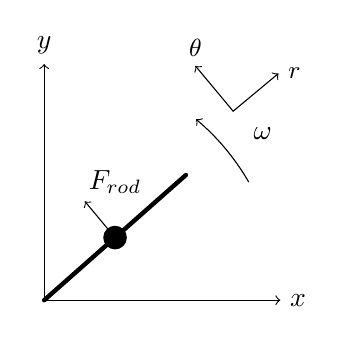
\begin{tikzpicture}[scale=3]
                    \draw[<->] (0,1) |- (1,0);
                    \draw[ultra thick,line cap=round] (0,0) -- (0.6,0.53);
                    \fill (0.3,0.265) circle [radius=0.05];
                    \draw[->,rotate=30] (1,0) arc [radius=1, start angle=0, end angle=20];
                    \draw[->,shift={(0.3,0.265)}, rotate=39.8] (0,0) -- (0,0.2);
                    \node[right] at (1,0) {$x$};
                    \node[above] at (0,1) {$y$};
                    \node at (0.3,0.5) {$F_\text{rod}$};
                    \node[right] at (39.8:1.1) {$\omega$};

                    \begin{scope}[shift={(0.8,0.8)},scale=0.25,rotate=39.8,font=\small]
                        \draw[<->] (0,1) |- (1,0);
                        \node[right] at (1,0) {$\uvec{r}$};
                        \node[above] at (0,1) {$\uvec{\theta}$};    
                    \end{scope}
                \end{tikzpicture}
            \end{figure}

            \paragraph{}
            Since the total force on the bead is $\vec{F}=F_\text{rod}\uvec{\theta}$, the instantaneous radial acceleration $a_r=\ddot{r}-r\dot{\theta}^2$ must be zero.
            This is a differential equation that we can solve for the radial motion.
            \begin{equation}
                \dv[2]{r}{t}-\omega^2r=0.
            \end{equation}
            Using an ansatz of the form $r=Ae^{Bt}$, with two unknown constants $A$ and $B$, we get
            \begin{align}
                &\dv[2]{}{t}(Ae^{Bt})-\omega^2Ae^{Bt}=0\\
                &AB^2e^{Bt}-\omega^2Ae^{Bt}=0\\
                &B^2-\omega^2=0.
            \end{align}
            This gives $B=\pm\omega$, so we get the general solution
            \begin{equation}
                r=A_+e^{\omega t}+A_-e^{-\omega t}.
            \end{equation}
            When $t=0$, $r$ is some value $r_0$ and $\dot{r}=0$, so
            \begin{align}
                \dot{r}(0)&=\left.A_+\omega e^{\omega t}-A_-\omega e^{-\omega t}\right|_{t=0}\\
                &=\omega(A_+-A_-)=0,
            \end{align}
            therefore $A_+=A_-=$, so we will relabel them both $A$.
            Finally, $r(0)=2A=r_0$, so we have
            \begin{align}
                r&=\frac{1}{2}r_0(e^{\omega t}+e^{-\omega t})\\
                &=r_0\cosh(\omega t).
            \end{align}
            % TODO: add plot of radial motion
        \end{example}

    \section{Constant Angular Acceleration}
        \paragraph{}
        In the case where we have a constant angular acceleration, we can derive a set of equations analogous to the SUVAT equations for linear motion derived in section~\ref{sec:suvat}.
        From the equation for average acceleration above, we get
        \begin{align}
            \Delta\omega=\omega(t)-\omega_0&=\alpha t\\
            \omega(t)&=\omega_0+\alpha t,\label{eq:ang-suvat-1}
        \end{align}
        which is analogous to equation~\ref{eq:suvat-1}.
        Then from the definition of angular displacement,
        \begin{align}
            \Delta\theta&=\int_{t_1}^{t_2}(\omega_0+\alpha t)\dd{t}\\
            &=\omega_0t+\frac{1}{2}\alpha t^2\\
            \implies\theta(t)&=\theta_0+\omega_0t+\frac{1}{2}\alpha t^2.\label{eq:ang-suvat-2}
        \end{align}
        This is like equation~\ref{eq:suvat-2}
        Finally, squaring equation~\ref{eq:ang-suvat-1} and substituting it into equation~\ref{eq:ang-suvat-2} gives the last equation:
        \begin{equation}
            \omega^2(t)=\omega_0^2+2\alpha\theta(t),\label{eq:ang-suvat-3}
        \end{equation}
        which is an angular version of equation~\ref{eq:suvat-3}.
        These equations are useful in solving problems where we don't have to worry (or don't care) about motion in the radial direction.

    \section{Uniform Circular Motion}
        % TODO: move this section to the beginning of this chapter?
        \paragraph{}
        The simplest case of angular motion is where an object is moving in a circle, so there is no motion in the radial direction, and going at a constant speed.
        This is called \textbf{uniform circular motion}, and objects moving this way can be analysed using 1D techniques we studied in section~\ref{sec:motion-in-1d}.
        \begin{figure}[H]
            \centering
            \begin{tikzpicture}[scale=3]
                \draw[->] (-1,0) -- (1,0);
                \draw[->] (0,-1) -- (0,1);
                \draw[dashed] (0,0) circle [radius=0.8];
                \draw[thick] (0,0) -- (0.6,0.53);
                \fill (0.6,0.53) circle [radius=0.02];
                \draw (0.2,0) arc [radius=0.2, start angle=0, end angle=39.8];
                \draw[->,rotate=30] (1,0) arc [radius=1, start angle=0, end angle=20];
                \node[right] at (1,0) {$x$};
                \node[above] at (0,1) {$y$};
                \node at (0.25,0.1) {$\theta$};
                \node[above] at (0.3,0.265) {$r$};
                \node[right] at (39.8:1.1) {$\dot{\theta}=\omega$};
            \end{tikzpicture}
        \end{figure}
        First, note that the displacement is the arc length of the circular path, given by $s=r\theta$, where $\theta$ is the angular displacement in radians and $r$ is the radius of the circle.
        Thus, the velocity along the path is given as
        \begin{equation}\label{eq:ucm-speed}
            v=\dv{s}{t}=r\dv{\theta}{t}=r\omega.
        \end{equation}
        Since the speed is constant, $\omega$ is constant as well.
        Therefore, by equation~\ref{eq:ang-suvat-2}, we have $\theta=\omega t$.

        \paragraph{}
        Does this mean acceleration is zero?
        No.
        Since $\omega$ is constant, $\alpha=\dot{\omega}=0$, but this does not mean that the linear acceleration is zero.
        Recall Newton's first law of motion, definition~\ref{def:newton-1}: if the \textit{velocity} is constant, the force (acceleration) is zero.
        Since the path of motion is a circle, the velocity vector is constantly changing direction and is therefore \textit{not} constant.

        \paragraph{}
        We will calculate the velocity and accelearation in cartesian coordinates first.
        Taking equation~\ref{eq:2d-polar-velocity-cartesian} and dropping the terms with $\dot{r}$, we get
        \begin{align}
            \vec{v}&=-r\omega\sin(\omega t)\ihat+r\omega\cos(\omega t)\jhat\\
            \vec{a}&=\dv{\vec{v}}{t}\\
            &=-r\omega^2\cos(\omega t)\ihat-r\omega^2\sin(\omega t)\jhat.
        \end{align}
        As a sanity check, we can see that the speed is given by
        \begin{align}
            \abs{\vec{v}}&=\sqrt{(-r\omega\sin(\omega t))^2+(r\omega\cos(\omega t))^2}\\
            &=\sqrt{r^2\omega^2(\sin^2(\omega t)+\cos^2(\omega t))}\\
            &=r\omega,
        \end{align}
        which is what we found before.
        It is not immediately clear in this coordinate system which direction the velocity points in, let's calculate the dot product with the position vector to find out.
        \begin{align}
            \vec{v}\cdot\vec{r}&=(-r\omega\sin(\omega t)\ihat+r\omega\cos(\omega t)\jhat)\cdot(r\cos(\omega t)\ihat+r\sin(\omega t)\jhat)\\
            &=-r^2\omega\sin(\omega t)\cos(\omega t)+r^2\omega\sin(\omega t)\cos(\omega t)\\
            &=0.
        \end{align}
        Hence the velocity and position vectors are perpendicular.
        This makes sense because as we know from section~\ref{sec:motion-in-2-3d}, the velocity is always tangent to the trajectory, which corresponds to being perpendicular to the position vector in the case of a circle.

        \paragraph{}
        Finally, notice that since $\vec{r}=r\sin(\omega t)\ihat+r\cos(\omega t)\jhat$,
        \begin{equation}
            \vec{a}=-\omega^2\vec{r}.
        \end{equation}
        The acceleration is antiparallel to the position vector, pointing in towards the centre of the circle.
        The magnitude of the acceleration is
        \begin{align}
            \abs{\vec{a}}&=\abs{-\omega^2}\abs{\vec{r}}\\
            &=r\omega^2\\
            &=\frac{v^2}{r},
        \end{align}
        where we have substituted equation~\ref{eq:ucm-speed} in the last line
        Thus the magnitude of the acceleration is constant, but the direction changes as the object moves on its circular path.
        By Newton's second law, a nonzero acceleration implies an unbalanced force.
        This force is what keeps the object moving on its circular path and is known as the \textbf{centripetal force}.
        It is given by
        \begin{equation}
            \vec{F}_\text{centripetal}=m\vec{a}=-mr\omega^2\uvec{r}=-\frac{mv^2}{r}\uvec{r}.
        \end{equation}

        \paragraph{}
        Let us see if we can reproduce these results using the 2D polar coordinate vectors.
        Using equation~\ref{eq:2d-polar-velocity} and noting that $r$ is constant, we immediately recover
        \begin{equation}
            \vec{v}=r\omega\uvec{\theta}.
        \end{equation}
        Here it is immediately apparent that the velocity always points perpendicular to the position vector.
        In equation~\ref{eq:2d-polar-acceleration}, any time derivatives of $r$ drop out, as well as $\ddot{\theta}$, leaving us with
        \begin{equation}
            \vec{a}=-r\dot{\theta}^2\uvec{r},
        \end{equation}
        which is the same as above.       
        
        \begin{example}
            Consider a child on a merry-go-round.
            If the platform is rotating at 60rpm and the child is holding on, what is the force on the child's arm?
            % TODO: complete this example
        \end{example}
        \begin{example}
            Consider a conical pendulum. 
            If the bob of mass of 200g on a string of length 50cm is swinging around at a frequency of 1 rotation per second, what is the angle that the pendulum makes with the vertical?
            % TODO: complete this example
        \end{example}
        \begin{example}
            Consider a car going round a circular bend.
            Find the maximum velocity that the car can take the bend at without skidding.
            % TODO: complete this example
        \end{example}
        \begin{example}
            Consider a ball rolling on a circular banked curve.
            What is the speed required to maintain a constant height on the curve as a function on the banking angle?
            % TODO: complete this example 
        \end{example}
        This next example uses the concept of energy conservation in combination with the traditional method of comparing forces to solve the problem.
        \begin{example}
            Consider a mass on a string.
            The mass starts hanging vertically downwards, then it gets projected sideways at a speed $v_0$.
            When the angle between the string and the vertical is $120^\circ$, the string becomes slack and the mass falls.
            Find the initial speed $v_0$ in terms of the length of the string.
            % TODO: complete this example
            First use energy conservation to relate the change in kinetic energy to the change in gravitational potential energy.
            % TODO: explain why this is valid since gravitational force is conservative and centripetal force doesn't change magnitude of velocity
            Then evaluate the forces at the top of the path to get a formula for the final velocity.
            Finally use the conservation of energy to solve for $v_0$.

            \paragraph{}
            How fast would the mass haves to be projected to get to the top of the loop?
        \end{example}

    \section{Rigid Body Rotation}
        \paragraph{}
        % TODO: introduce moment of inertia for a single particle first
        A rigid body is a system of particles which are fixed together such that they move together, no matter the forces applied.
        We have seen in previous chapters that it is possible to treat rigid bodies as point masses when considering linear motion.
        However, when considering rotational effects as well, we need to consider the macroscopic extent of an object.
        Consider a rigid body in motion and look at the total kinetic energy, which is given by the sum of kinetic energy of each constituent particle:
        \begin{equation}
            K=\sum_i\frac{1}{2}m_i\vec{v}_i\cdot\vec{v}_i.
        \end{equation}
        We can split the velocity of each particle into the sum of velocity around the centre of rotation and velocity along the line of motion.
        \begin{align}
            K&=\sum_i\frac{1}{2}m_i(\vec{v}_{i,\text{rot}}+\vec{v}_{i,\text{lin}})^2\\
            &=\sum_i\frac{1}{2}m_i(v_{i,\text{rot}}^2+v_{i,\text{lin}}^2+2\vec{v}_{i,\text{rot}}\cdot\vec{v}_{i,\text{lin}})\\
            &=\underbrace{\sum_i\frac{1}{2}m_iv_{i,\text{rot}}^2}_{K_\text{rotational}}+\underbrace{\sum_i\frac{1}{2}m_iv_{i,\text{lin}}^2}_{K_\text{linear}}.
        \end{align}
        The cross-term in the square cancels out (why?).
        % TODO: explain this fully
        % TODO: include a diagram of this
        Assuming the rigid body is rotating about a \textit{fixed} axis, all particles rotate in circles with the same angular velocity $\omega$ because their distance from the axis of rotation is constant.
        This means the rotational kinetic energy can be written as
        \begin{align}
            K_\text{rot}&=\sum_i\frac{1}{2}m_iv_{i,\text{rot}}^2=\sum_i\frac{1}{2}m_i(r_i\omega)^2\\
            &=\frac{1}{2}\omega^2\sum_i m_ir_i^2\\
            &=\frac{1}{2}I\omega^2.
        \end{align}
        $I$ is called the \textbf{moment of inertia}, and it is kind of an angular equivalent of mass.
        Notice how it is calculated in a similar way to the centre of mass except with the square of $r$.
        Also notice how in the formula for $K_\text{rot}$, $I$ and $\omega$ play the role of $m$ and $v$ respectively, which shows how they are analogous to the linear quantities.
        However $I$, just like the centre of mass, depends on how the mass is distributed in an object.
        For example, consider a solid disc and a hoop of the same mass.
        % TODO: include a diagram for this
        From the formula for $I$, we can see that since all of the mass in the hoop is concentrated further out, the moment of inertia will be larger than the disc.
        This means that for the same angular velocity, the rotational kinetic energy of the hoop will be larger than the disc.
        $I$ also depends on the axis of rotation, since a different axis will have a different mass distribution around it.

        \paragraph{}
        Let's do a few examples of calculating moments of inertia.
        \begin{example}
            Consider a system of two particles with masses $m_1$ and $m_2$ separated by a distance $d$.
            \begin{figure}[H]
                \centering
                \begin{tikzpicture}[scale=3]
                    \draw[dashed] (0,-0.5) -- (0,0.5);
                    \draw[dashed] (0.5,-0.5) -- (0.5,0.5);
                    \node[below right] at (0,0.5) {$A$};
                    \node[below right] at (0.5,0.5) {$B$};
                    \fill (0,0) circle [radius=0.02];
                    \fill (1,0) circle [radius=0.02];
                    \node[above left] at (0,0) {$m_1$};
                    \node[above right] at (1,0) {$m_2$};
                    \draw[<->] (0,-0.2) -- (1,-0.2);
                    \node[below right] at (0.5,-0.2) {$d$};
                \end{tikzpicture}
            \end{figure}
            What is the moment of inertia about the axis which passes through $m_1$ ($A$) and about the axis which passes halfway between $m_1$ and $m_2$ ($B$)?

            \paragraph{}
            Lets to the axis which runs through the midpoint first.
            Using the formula for moment of inertia, we get
            \begin{align}
                I_B&=m_1r_1^2+m_2r_2^2\\
                &=m_1\left(\frac{d}{2}\right)^2+m_2\left(\frac{d}{2}\right)^2\\
                &=\frac{m_1+m_2}{4}d^2.
            \end{align}
            For the moment of inertia about axis $A$, the distance of $m_1$ from the axis is zero, so the moment of inertia is
            \begin{equation}
                I_A=m_2 d^2.
            \end{equation}
            The key takeaway here is that any mass located at the axis of rotation contributes \textit{nothing} to the moment of inertia, no matter how much it is.
        \end{example}

        \paragraph{}
        Just like calculating the centre of mass, when we have a continuous body we have to calculate moments of inertia using integrals.
        The formula is then
        \begin{equation}
            I=\int r^2\dd{m},
        \end{equation}
        where we have to find a way to express the mass element $\dd{m}$ in terms of length, area, or volume elements. 
        We will now find the moments of inertia of common shapes.
        \begin{example}
            Find the moment of inertia of a thin rod of uniform density rotating about its midpoint.
            % TODO: add diagram for this including mass element on the diagram
            % \begin{figure}[H]
            %     \centering
            %     \begin{tikzpicture}
                    
            %     \end{tikzpicture}
            % \end{figure}

            \paragraph{}
            Let $L$ be the length of the rod and $\lambda$ be its linear mass density.
            Then from the diagram, we can see that $\dd{m}=\lambda\dd{x}$.
            For the integral, the limits are $-L/2$ and $L/2$ and $r^2=x^2$, so we have
            \begin{equation}
                I=\int_{\frac{L}{2}}^{\frac{L}{2}}x^2\lambda\dd{x}=\left.\frac{\lambda x^3}{3}\right|_{\frac{L}{2}}^{\frac{L}{2}}=\frac{\lambda L^3}{12}.
            \end{equation}
            If we let $M$ be the total mass then $M=\lambda L$, and we have
            \begin{equation}
                I=\frac{1}{12}ML^2.
            \end{equation}
        \end{example}
        \begin{example}
            Find the moment of inertia of a uniform density thin hoop of radius $r$ in the $x$-$y$ plane rotating around the $z$-axis about its centre.
            % TODO: add diagram for this including mass element on the diagram
            % \begin{figure}[H]
            %     \centering
            %     \begin{tikzpicture}
                    
            %     \end{tikzpicture}
            % \end{figure}

            \paragraph{}
            We can use a symmetry argument to solve this.
            The distance from the axis is constant, so it doesn't change for any mass element and can be taken out of the integral.
            Thus the moment of inertia just the total mass multiplied by the radius squared.
            \begin{equation}
                I=Mr^2.
            \end{equation}
            Note that this is the same result as a point mass of mass $M$ revolving around the $z$-axis at the same radius $r$. 
        \end{example}
        \begin{example}
            Find the moment of inertia of a uniform density thin disc of radius $R$ in the $x$-$y$ plane rotating about the $z$-axis about its centre.
            % TODO: add diagram for this including mass element on the diagram
            % \begin{figure}[H]
            %     \centering
            %     \begin{tikzpicture}
                    
            %     \end{tikzpicture}
            % \end{figure}
            Here, we can use the result from the thin hoop.
            If we split the disc up into thin hoops, then we have $\dd{I}=r^2\dd{m}$ and we can integrate this from $0$ to $R$.
            But first, we need to write the mass element in terms of the radius of the thin hoop.
            We can write $\dd{m}=\mu\dd{A}$ where $\mu$ is the surface density of the disc, and the area of a thin hoop is $\dd{A}=2\pi r\dd{r}$.
            Putting this all together, we get
            \begin{align}
                I=\int_0^R 2\pi\mu r^3\dd{r}=\left.\frac{2\pi\mu r^4}{4}\right|_0^R=\frac{1}{2}\pi\mu R^4.
            \end{align}
            The total mass of the disc is $M=\mu A=\mu\pi R^2$, so this simplifies to
            \begin{equation}
                I=\frac{1}{2}MR^2.
            \end{equation}
            So the moment of inertia of a thin disc is half that of a thin hoop with the same mass and radius.
        \end{example}
        \begin{example}
            Find the moment of inertia of a uniform density sphere of radius $R$ rotating about its centre.
            % TODO: add diagram for this including mass element on the diagram and diagram of cross-section
            % \begin{figure}[H]
            %     \centering
            %     \begin{tikzpicture}
                    
            %     \end{tikzpicture}
            % \end{figure}
            Here we will again build upon previous results, this time using the moment of inertia of a thin disc.
            By aligning the axis of rotation with the $z$-axis, we can split the sphere into thin discs of different radii and at different heights on the $z$-axis.
            Then the total moment of inertia is found by integrating over $\dd{I}=\frac{1}{2}r^2\dd{m}$, where $r$ is the radius of the thin disc.
            $\dd{m}$ is given by $\rho\dd{V}$ where $\rho$ is the volume density, and the volume element $\dd{V}$ is the area of the disc multiplied by its height, $\dd{V}=\pi r^2\dd{z}$.
            So far, we have
            \begin{equation}
                \dd{I}=\frac{1}{2}\rho\pi r^4\dd{z}.
            \end{equation}
            In order to integrate this we need a relation between $r$, the radius of each disc, and $z$, its height.
            This is given by Pythagoras' theorem (see the diagram above) as $r^2=R^2-z^2$ so we get
            \begin{equation}
                \dd{I}=\frac{1}{2}\rho\pi(R^2-z^2)^2\dd{z}.
            \end{equation}
            We can now tackle the integral:
            \begin{align}
                I&=\int_{-R}^{R}\frac{1}{2}\rho\pi(R^2-z^2)^2\dd{z}\\
                &=\int_0^R\rho\pi(R^4+z^4-2R^2z^2)\dd{z}\\
                &=\rho\pi\left[R^4z+\frac{z^5}{z}-\frac{2}{3}R^2z^3\right]_0^R\\
                &=\frac{8}{15}\rho\pi R^5.
            \end{align}
            Note that in the second line we have used symmetry to ignore half of the integral and double the result.
            The mass of a sphere is $M=\frac{4}{3}\rho\pi R^3$, so we have
            \begin{equation}
                I=\frac{2}{5}MR^2.
            \end{equation}
        \end{example}

        \paragraph{}
        We will now look at two useful results that help with calculating more moments of inertia.
        \begin{theorem}[Parallel Axis Theorem]
            For a system of total mass $M$ and moment of inertia about an axis passing through the centre of mass $I_\text{COM}$, the moment of inertia about a parallel axis a distance $d$ away is
            \begin{equation}
                I_\parallel=I_\text{COM}+Md^2.
            \end{equation}
            % TODO: include diagram for this
        \end{theorem}
        \begin{proof}
            Let's put ourselves in the centre of mass frame, align the $z$-axis with the axis of rotation and the $x$-axis with the along the perpendicular distance between the two axes.
            The moment of inertia relative to the $z$-axis is
            \begin{equation}
                I_\text{COM}=\int(x^2+y^2)\dd{m},
            \end{equation}
            and the moment of inertia relative to the other axis is
            \begin{align}
                I_\parallel&=\int[(x-d)^2+y^2]\dd{m}\\
                &=\int(x^2+y^2)\dd{m}+d^2\int\dd{m}+2d\int x\dd{m}\\
                &=I_\text{COM}+Md^2+2d\int x\dd{m}.
            \end{align}
            The integral in the last term is $x$ coordinate of the centre of mass, which is zero in the centre of mass frame.
            So the last term disappears, leaving us with the result.
        \end{proof}

        \paragraph{}
        We can use this result to calculate moments of inertia of shapes we have seen before about different axes that might be difficult to find via a straightforward approach.
        \begin{example}
            Consider a uniform density thin disc of radius $R$ in the $x$-$y$ plane, but instead of rotating around the $z$-axis about its centre like before, it is rotating about a point on the circumference.
            % TODO: include diagram for this
            
            \paragraph{}
            We know that the moment of inertia of the thin disc about the centre is $I_\text{COM}=\frac{1}{2}MR^2$, and the distance to the parallel axis is simply the radius $R$, so applying the parallel axis theorem we get
            \begin{equation}
                I_\parallel=\frac{1}{2}MR^2+MR^2=\frac{3}{2}MR^2.
            \end{equation}
        \end{example}
        \begin{theorem}[Perpendicular Axis Theorem]
            Suppose we have a planar lamina lying in the $x$-$y$ plane.
            The moment of inertia about the $z$ axis, $I_z$, is related to the moments of inertia about the $x$ and $y$-axes, $I_x$ and $I_y$, by
            \begin{equation}
                I_z=I_x+I_y.
            \end{equation}
        \end{theorem}
        \begin{proof}
            The proof is straightforward: manipulating the integral for moment of inertia about the $z$-axis we get
            \begin{equation}
                I_z=\int(x^2+y^2)\dd{m}=\int x^2\dd{m}+\int y^2\dd{m}=I_y+I_x.
            \end{equation}
            Note that $\int x^2\dd{m}=I_y$, not $I_x$ since $x^2$ in this case denotes the perpendicular distance from the axis of rotation, which must be around the $y$-axis.
        \end{proof}
        \begin{example}
            Consider the uniform density thin disc again.
            What is its moment of inertia about the $x$ and $y$ axes?
            % TODO: include diagram for this

            \paragraph{}
            We know that $I_z=\frac{1}{2}MR^2$ for the thin disc, and by the perpendicular axis theorem we have $I_z=I_x+I_y$.
            In this case we can invoke symmetry of the disc to argue that $I_x=I_y$, and therefore $I_z=2I_x=2I_y$.
            Therefore we must have
            \begin{equation}
                I_x=I_y=\frac{I_z}{2}=\frac{1}{4}MR^2.
            \end{equation}
        \end{example}
        \begin{theorem}[Stretch Rule]
            The moment of inertia of a rigid object is unchanged when the object is stretched parallel to the axis of rotation and the distribution of mass is kept the same (except along the axis of rotation).
            This allows us to take a planar object and extrude it into 3D along the $z$-axis while keeping the same mass and moment of inertia.
        \end{theorem}
        \begin{proof}
            Have an object of cross-sectional area in the $x$-$y$ plane $A$ and height $L$.
            Then the moment of inertia around the $z$-axis can be expressed as
            \begin{equation}
                I_z=\int(x^2+y^2)\rho(x,y,z)\dd{V}=\int_0^L\dd{z}\int_A(x^2+y^2)\rho(x,y,z)\dd{A}.
            \end{equation}
            If we stretch this object along $z$ by a factor of $a$, then we have to divide the mass density by $a$ and change the upper limit on the $z$ integral to the new height $aL$.
            This means the total mass remains unchanged.
            Then the new moment of inertia is
            \begin{equation}
                I_z^\prime=\int_0^{aL}\dd{z}\int_A(x^2+y^2)\frac{\rho(x,y,z/a)}{a}\dd{A}.
            \end{equation}
            Making the substitution $z^\prime=z/a$, we get
            \begin{align}
                I_z^\prime&=\int_0^L a\dd{z}^\prime\int_A(x^2+y^2)\frac{\rho(x,y,z^\prime)}{a}\dd{A}\\
                &=\int_0^L\dd{z}^\prime\int_A(x^2+y^2)\rho(x,y,z^\prime)\dd{A}\\
                &=I_z.
            \end{align}
        \end{proof}
        Using the stretch rule, we can say that the moment of inertia of a cylinder rotating about its main axis is the same as a thin disc.
        % TODO: link to wikipedia lists of moments of inertia

        \paragraph{}
        Let's now look at some problems which combine all the ideas of this chapter.
        \begin{example}
            % TODO: change this example to block falling from a pulley, find a formula for the velocity, acceleration of the block
            % a = g/(1+m_reel/(2m_block))
            % v = sqrt(2gh/(1+m_reel/(2m_block)))
            A light inextensible cable is being pulled out from a reel with a force of \qty{9}{\newton}.
            The reel weighs \qty{50}{\kilogram} and has a radius of \qty{0.6}{\meter}.
            After \qty{2}{\meter} of the cable have been pulled out, what it its velocity?
            \begin{figure}[H]
                \centering
                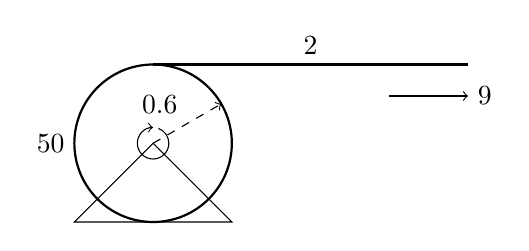
\begin{tikzpicture}
                    \draw[very thick] (0,1) -- (4,1);
                    \node[above] at (2,1) {\qty{2}{\meter}};

                    \draw[->] (3,0.6) -- (4,0.6);
                    \node[right] at (4,0.6) {\qty{9}{\newton}};

                    \draw[thick] (0,0) circle [radius=1];
                    \draw (0,0) -- (-1,-1) -- (1,-1) -- cycle;
                    \draw[<-,rotate=90] (0.2,0) arc [radius=0.2, start angle=0, end angle=340];
                    \node[left] at (-1,0) {\qty{50}{\kilogram}};

                    \draw[->,dashed] (0,0) -- (0.866,0.5);
                    \node[above left] at (0.433,0.25) {\qty{0.6}{\meter}};
                \end{tikzpicture}
            \end{figure}
            
            \paragraph{}
            To solve this, we will look at the rotational kinetic energy of the pulley before and after and then invoke the work-energy theorem.
            Its initial kinetic energy is zero, and its final kinetic energy is its rotational kinetic energy $K_\text{rot}=\frac{1}{2}I\omega^2$.
            By the work-energy theorem, the final kinetic energy is equal to the work done, which is the length of rope pulled out multiplied by the tension $W=Ts$.
            Putting these two equations together and rearranging for $\omega$, we get
            \begin{equation}
                \omega=\sqrt{\frac{2Ts}{I}}.
            \end{equation}
            By the stretch rule, the moment of inertia of the reel is the same as a thin disc, namely $I=\frac{1}{2}MR^2$, so we get
            \begin{equation}
                \omega=\sqrt{\frac{4Ts}{MR^2}}=\sqrt{\frac{4\cdot\qty{9}{\newton}\cdot\qty{2}{\meter}}{\qty{50}{\kilogram}\cdot(\qty{0.6}{\meter})^2}}=\qty{2}{\radian\per\second}.
            \end{equation}
            Now that we have the final angular velocity of the reel, the speed of the cable is just the tangential speed of the reel at its edge, which is
            \begin{equation}
                v_\text{cable}=v_\text{reel}=R\omega=\qty{0.6}{\meter}\cdot\qty{2}{\radian\per\second}=\qty{1.2}{\meter\per\second}.
            \end{equation}
        \end{example}
        \begin{example}
            Suppose a dumbbell-shaped pendulum is allowed to fall from horizontal.
            The weights at each end are spherical with radius $r=\qty{10}{\centi\meter}$ and they weigh $m_\text{weight}=\qty{10}{\kilogram}$.
            The bar is $l=\qty{60}{\centi\meter}$ long and weighs $m_\text{bar}=\qty{1}{\kilogram}$.
            The pivot point is at the left end of the bar.
            What is angular velocity of the dumbbell when it is vertical?
            \begin{figure}[H]
                \centering
                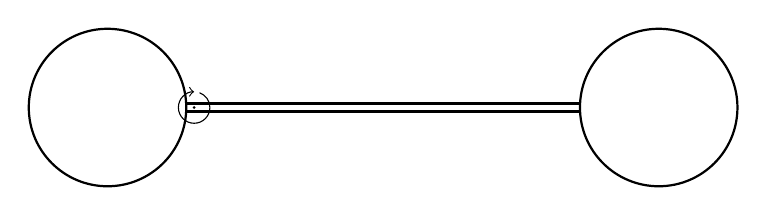
\begin{tikzpicture}
                    % TODO: add labels to diagram
                    \draw[thick] (0,0) circle [radius=1];
                    \draw[thick] (1,-0.05) -- (1,0.05) -- (6,0.05) -- (6,-0.05) -- cycle;
                    \draw[thick] (7,0) circle [radius=1];

                    \draw (1.1,0) circle [radius=0.01];
                    \draw[<-,rotate=90,shift={(0,-1.1)}] (0.2,0) arc [radius=0.2, start angle=0, end angle=340];
                \end{tikzpicture}
            \end{figure}
            
            \paragraph{}
            The first step to solving this problem is working out the moment of inertia of the dumbbell about the pivot point.
            If we split the dumbbell into the two weights ($A$ for the one above the pivot and $B$ for the one below) and the bar, the total moment of inertia can be written as
            \begin{equation}
                I=I_A+I_\text{bar}+I_B.
            \end{equation}
            Using the parallel axis theorem, the moment of inertia of the bar is $I_\text{bar}=\frac{1}{12}m_\text{bar}l^2+m_\text{bar}\left(\frac{1}{2}l\right)^2=\frac{1}{3}m_\text{bar}l^2$.
            For the weights, we can again use the parallel axis theorem since we know that the moment of inertia of a sphere is $\frac{2}{5}mr^2$.
            Hence we get
            \begin{align}
                I&=\left(\frac{2}{5}m_\text{weight}r^2+m_\text{weight}r^2\right)+\frac{1}{3}m_\text{bar}l^2+\left(\frac{2}{5}m_\text{weight}r^2+m_\text{weight}(l+r)^2\right)\\
                &=\frac{9}{5}\cdot\qty{10}{\kilogram}\cdot(\qty{0.1}{\meter})^2+\frac{1}{3}\cdot\qty{1}{\kilogram}\cdot(\qty{0.6}{\meter})^2+\qty{10}{\kilogram}\cdot(\qty{0.7}{\meter})^2\\
                &=\qty{5.2}{\kilogram\meter\squared}.
            \end{align}
            Now, to use energy conservation we also need to know the potential energy difference.
            To do this we need to know where the centre of mass is, since the potential energy difference is just $-Mgh$, where $M$ is the total mass and $h$ is the distance that the centre of mass dropped.
            % TODO: justify why this is the case?
            By symmetry, the centre of mass is clearly just the centre of the dumbbell which is a distance of \qty{30}{\centi\meter} from the pivot.
            Thus the height by which the centre of mass has dropped when it reaches the bottom is \qty{30}{\centi\meter}.
            Setting the zero point of the potential energy to be the initial height, the total energy before is zero since the dumbbell is not moving.
            The final energy is
            \begin{equation}
                E_f=\frac{1}{2}I\omega^2-Mgh=0.
            \end{equation}
            Rearranging for $\omega$, we get
            \begin{align}
                \omega&=\sqrt{\frac{2Mgh}{I}}\\
                &=\sqrt{\frac{2\cdot\qty{21}{\kilogram}\cdot\qty{9.8}{\meter\per\second\squared}\cdot\qty{0.3}{\meter}}{\qty{5.2}{\kilogram\meter\squared}}}\\
                &=\qty{4.87}{\radian\per\second}.
            \end{align}
        \end{example}

\end{document}
